% =============================================================================
% Section 8 — Topological Data Analysis of Genomic Sequence
% =============================================================================
\section{Topology of a Genome: Persistent Homology on Real Sequence}\label{sec:tda}

\begin{objectives}
\begin{itemize}[leftmargin=*,itemsep=1pt,topsep=1pt]
  \item Embed a DNA sequence as a point cloud whose geometry encodes $k$-mer context.
  \item Define a filtration and read birth--death pairs from a persistence diagram.
  \item Compute Betti numbers on a real coding sequence with GUDHI.
  \item Judge honestly when a topological feature is signal and when it is an artefact of the embedding.
\end{itemize}
\end{objectives}

\subsection{Why topology, and when not}

Topological data analysis asks what shape a dataset has at every scale at once.
Applied carelessly to biology it produces impressive pictures and no knowledge,
so this section is as much about restraint as about method. We compute real
persistent homology on a real sequence, and then we ask what it establishes ---
and the honest answer turns out to be narrower than the picture suggests.

\subsection{From sequence to point cloud}

A sequence of letters has no geometry until we give it one. The classical device
is the \textbf{chaos game representation}.

\begin{definition}[Chaos game representation, 3D]\label{def:cgr}
Assign the four bases to the vertices of a regular tetrahedron,
$v_A, v_C, v_G, v_T \in \mathbb{R}^3$. Start at the origin, $x_0 = 0$, and for
each successive base $b_i$ set
\begin{equation}\label{eq:cgr}
  x_i \;=\; \tfrac{1}{2}\left(x_{i-1} + v_{b_i}\right).
\end{equation}
\end{definition}

The construction has a property that makes it useful rather than decorative:
after $k$ steps the influence of $x_{i-k}$ is scaled by $2^{-k}$. Two positions
in the sequence therefore land close together exactly when they share a recent
suffix. Proximity in the cloud \emph{is} shared $k$-mer context, with longer
shared context giving closer points. The embedding is not arbitrary; it is a
geometric encoding of word statistics.

\subsection{Filtration and persistence}

\begin{definition}[Vietoris--Rips filtration]
For a finite point set $X \subset \mathbb{R}^3$ and $\epsilon \ge 0$, the complex
$\mathrm{VR}_\epsilon(X)$ has a simplex on every subset of diameter at most
$\epsilon$. As $\epsilon$ grows the complexes nest, and a homology class born at
$\epsilon_b$ and dying at $\epsilon_d$ is recorded as the pair
$(\epsilon_b, \epsilon_d)$.
\end{definition}

The quantity $\epsilon_d - \epsilon_b$ is the feature's \emph{persistence}. The
working assumption of TDA is that long bars are structure and short bars are
noise. That assumption is exactly what needs checking in any application.

\subsection{Computation on the \texttt{POLE} coding sequence}

\begin{numerics}[8.1]
\file{scripts/textbook/make_figures.py}, section~8. The canonical \texttt{POLE}
coding sequence is fetched from Ensembl ($6861$~nt), embedded by
\eqref{eq:cgr}, and subsampled to $900$ points. Persistent homology is computed
with GUDHI~3.13.0, Vietoris--Rips, maximum edge length $0.9$, up to dimension~2.

\medskip
\begin{tabularx}{\linewidth}{@{}l r X@{}}
\toprule
coding sequence length & $6861$ nt & Ensembl canonical transcript \\
points after subsampling & $900$ & uniform stride \\
Betti numbers $(\beta_0, \beta_1)$ & $(1, 0)$ & at the filtration limit \\
longest $H_1$ bar & $(0.171,\ 0.755)$ & persistence $0.584$ \\
\bottomrule
\end{tabularx}
\end{numerics}

\begin{figure}[htbp]
  \centering
  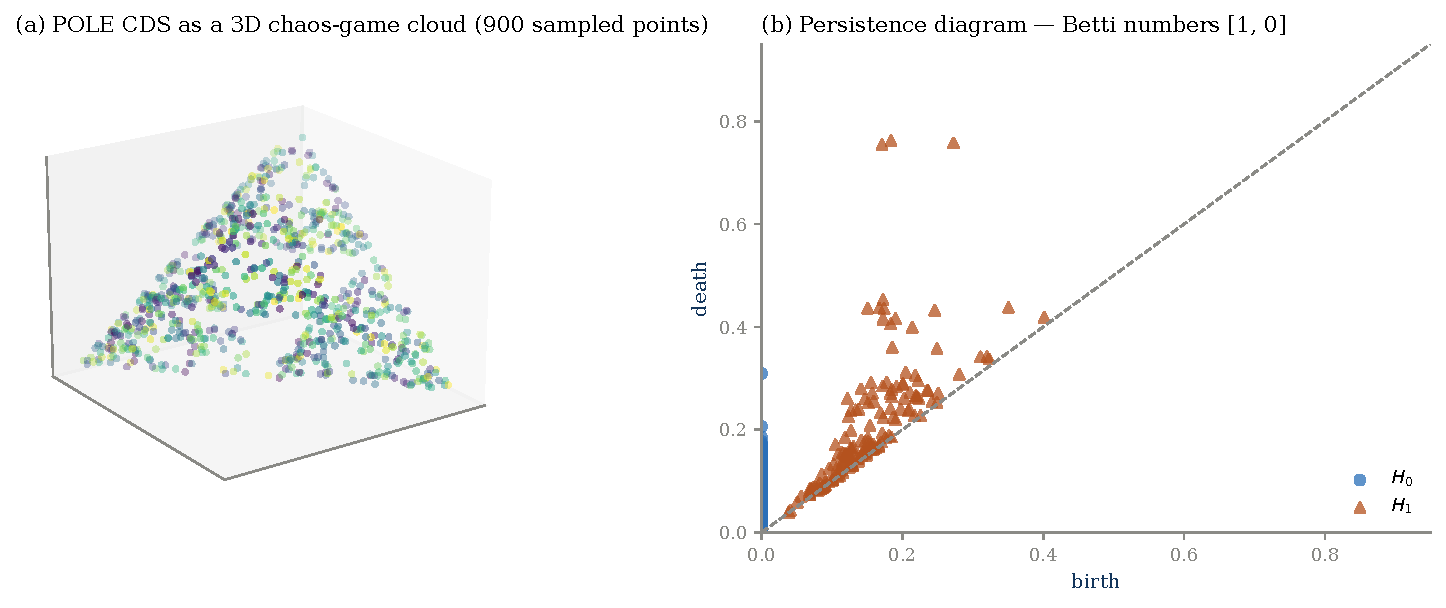
\includegraphics[width=\textwidth]{fig08_topological_genomics.pdf}
  \caption{(a) The \texttt{POLE} coding sequence as a chaos-game point cloud in
  $\mathbb{R}^3$, coloured by position along the transcript. The tetrahedral
  self-similar structure is the signature of \eqref{eq:cgr}. (b) The persistence
  diagram. Points far from the diagonal are long-lived features; $H_1$ classes
  are born and die well inside the filtration, leaving $\beta_1 = 0$ at the limit.}
  \label{fig:tda}
\end{figure}

\subsection{Reading the result honestly}

The cloud is connected ($\beta_0 = 1$) and has no surviving loops
($\beta_1 = 0$). There are, however, $H_1$ classes of substantial persistence ---
the longest living from $\epsilon = 0.171$ to $\epsilon = 0.755$.

Now the question that matters: \emph{is that a fact about \texttt{POLE}?}

It is largely a fact about the chaos game. The map \eqref{eq:cgr} sends any
sequence into a self-similar attractor --- the tetrahedral Sierpiński gasket ---
whose holes exist regardless of what the sequence says. A random sequence
produces loops of comparable persistence. So the bare Betti numbers of a single
sequence carry almost no biological information, and reporting them as though
they did would be precisely the overclaiming this book is organised against.

\begin{remark}[What would make this informative]
TDA becomes informative here under \emph{comparison}, not in isolation. The
honest designs are:
\begin{enumerate}[leftmargin=*,itemsep=1pt]
  \item \textbf{Against a null.} Compare the persistence of the real sequence
        with an ensemble of shuffles preserving mononucleotide --- or better,
        dinucleotide --- composition. A feature is evidence only if it exceeds
        that null.
  \item \textbf{Between sequences.} Compare persistence landscapes of orthologous
        genes, or of coding against non-coding regions, where the embedding
        artefact is common to both and cancels.
\end{enumerate}
This book computes neither. Figure~\ref{fig:tda} is therefore offered as a
\emph{method demonstration}, and the ledger records it as such. A reader who
wanted a biological claim from TDA should regard this section as the setup, not
the result.
\end{remark}

\begin{worked}[8.1: why the subsampling stride matters]
\textbf{Problem.} The computation subsamples $6861$ points down to $900$ by
uniform stride. Why not use all points, and what does the stride risk?

\textbf{Solution.} Vietoris--Rips on $n$ points builds up to $\binom{n}{3}$
triangles at dimension~2; at $n = 6861$ that is $5\times10^{10}$ simplices, which
is not computable here. Subsampling is a necessity, not a refinement.

The risk is specific: a uniform stride of $7$ interacts with the codon structure
of a coding sequence, whose period is $3$. A stride sharing a factor with the
reading frame can systematically over-sample one codon position. Here
$\gcd(7, 3) = 1$, so the three positions are sampled evenly --- but the check is
necessary, and a stride of $6$ or $9$ would have introduced a frame bias
invisible in the final diagram. Artefacts of this kind are the normal failure
mode of applied topology.
\end{worked}

\begin{exercise}
Show from \eqref{eq:cgr} that $x_i$ depends on $b_{i-k}$ with weight $2^{-k}$,
and deduce that two positions sharing a suffix of length $k$ lie within
$2^{-k}\,\mathrm{diam}$ of each other.
\end{exercise}

\begin{exercise}
Explain why $\beta_0 = 1$ at the filtration limit is uninformative for any
sufficiently long sequence. What value of the maximum edge length would make
$\beta_0$ informative, and what would it then be measuring?
\end{exercise}

\begin{exercise}
Design the shuffle null described in the remark. State precisely what is
preserved by your shuffle and what is destroyed, and say which biological
hypothesis each choice would let you test.
\end{exercise}

\begin{exercise}[(harder)]
Persistence diagrams can be compared with the bottleneck distance. Look up its
definition and explain why it is stable --- small perturbations of the point
cloud produce small changes in the diagram. Why is that stability a prerequisite
for using TDA on noisy biological data at all?
\end{exercise}

\begin{ledger}
\textbf{Measured:} the \texttt{POLE} canonical coding sequence, $6861$~nt,
retrieved from Ensembl and cached with its URL. The persistence computation is
exact given the point cloud (GUDHI~3.13.0). \\
\textbf{Assumed:} that the chaos-game embedding is a meaningful geometry for
sequence, and that Vietoris--Rips persistence on a $900$-point subsample
represents the full cloud. \\
\textbf{Proved:} nothing formalised. The Betti numbers are a computation, not a
theorem, and they are reported as a method demonstration. \\
\textbf{Open:} everything that would make this biological --- the shuffle null,
the cross-sequence comparison. Neither is performed in this book, and no claim
about \texttt{POLE} should be drawn from Figure~\ref{fig:tda}.
\end{ledger}
